\section{Tests at Statkraft's power plants Paper IV}
\begin{frame}
	\frametitle{Motivation}
	\begin{itemize}
		\item Relate the results from Paper III and the new requirements.
		\item Test the methods on more real datasets.
		\item Demonstrate that industry proposed tests can be done easier.
		\item Less theoretical presentation in a more industry focused conference.
	\end{itemize}
\end{frame}
\begin{frame}
	\frametitle{Power plant location}
	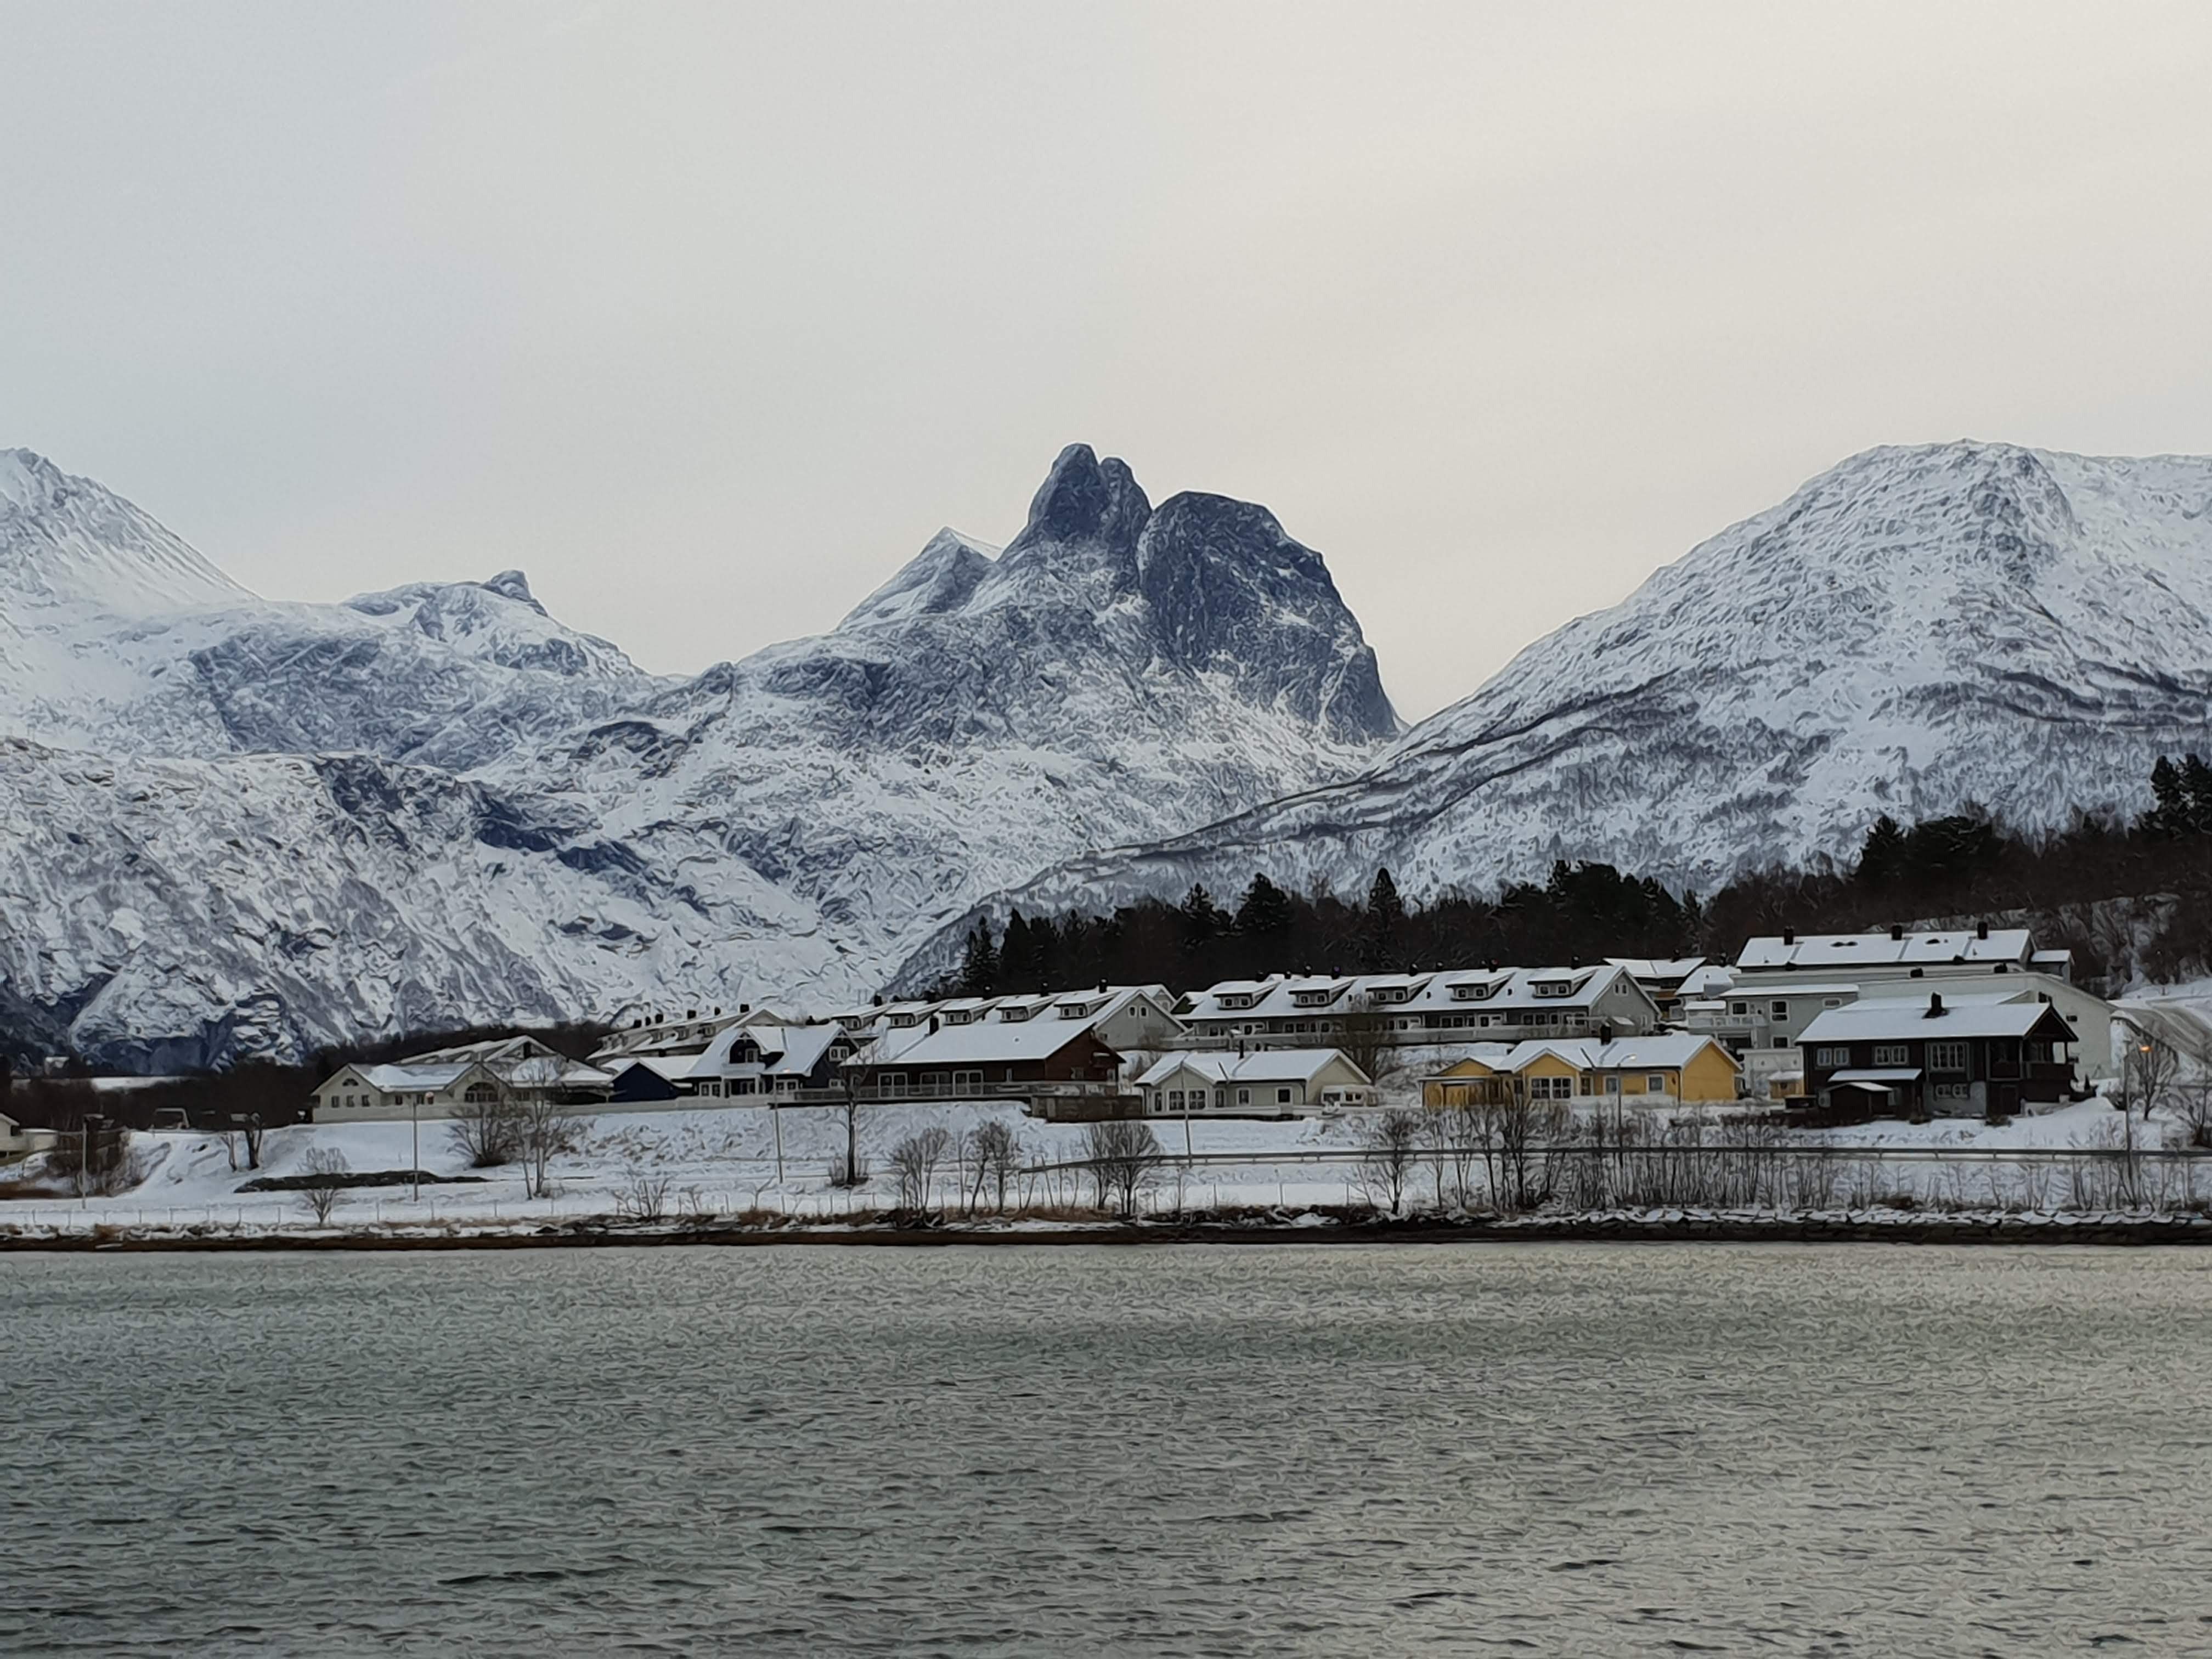
\includegraphics[width=\textwidth]{./pictures/romsdalshorn.jpg}
\end{frame}
\begin{frame}
	\frametitle{Getting data from the control system}
	\begin{columns}
		\begin{column}{0.3\textwidth}
			\begin{itemize}
					\item Collected Electric power $\Delta P_e$
				\item and power system frequency $f$.
			\end{itemize}
		\end{column}
		\begin{column}{0.7\textwidth}
			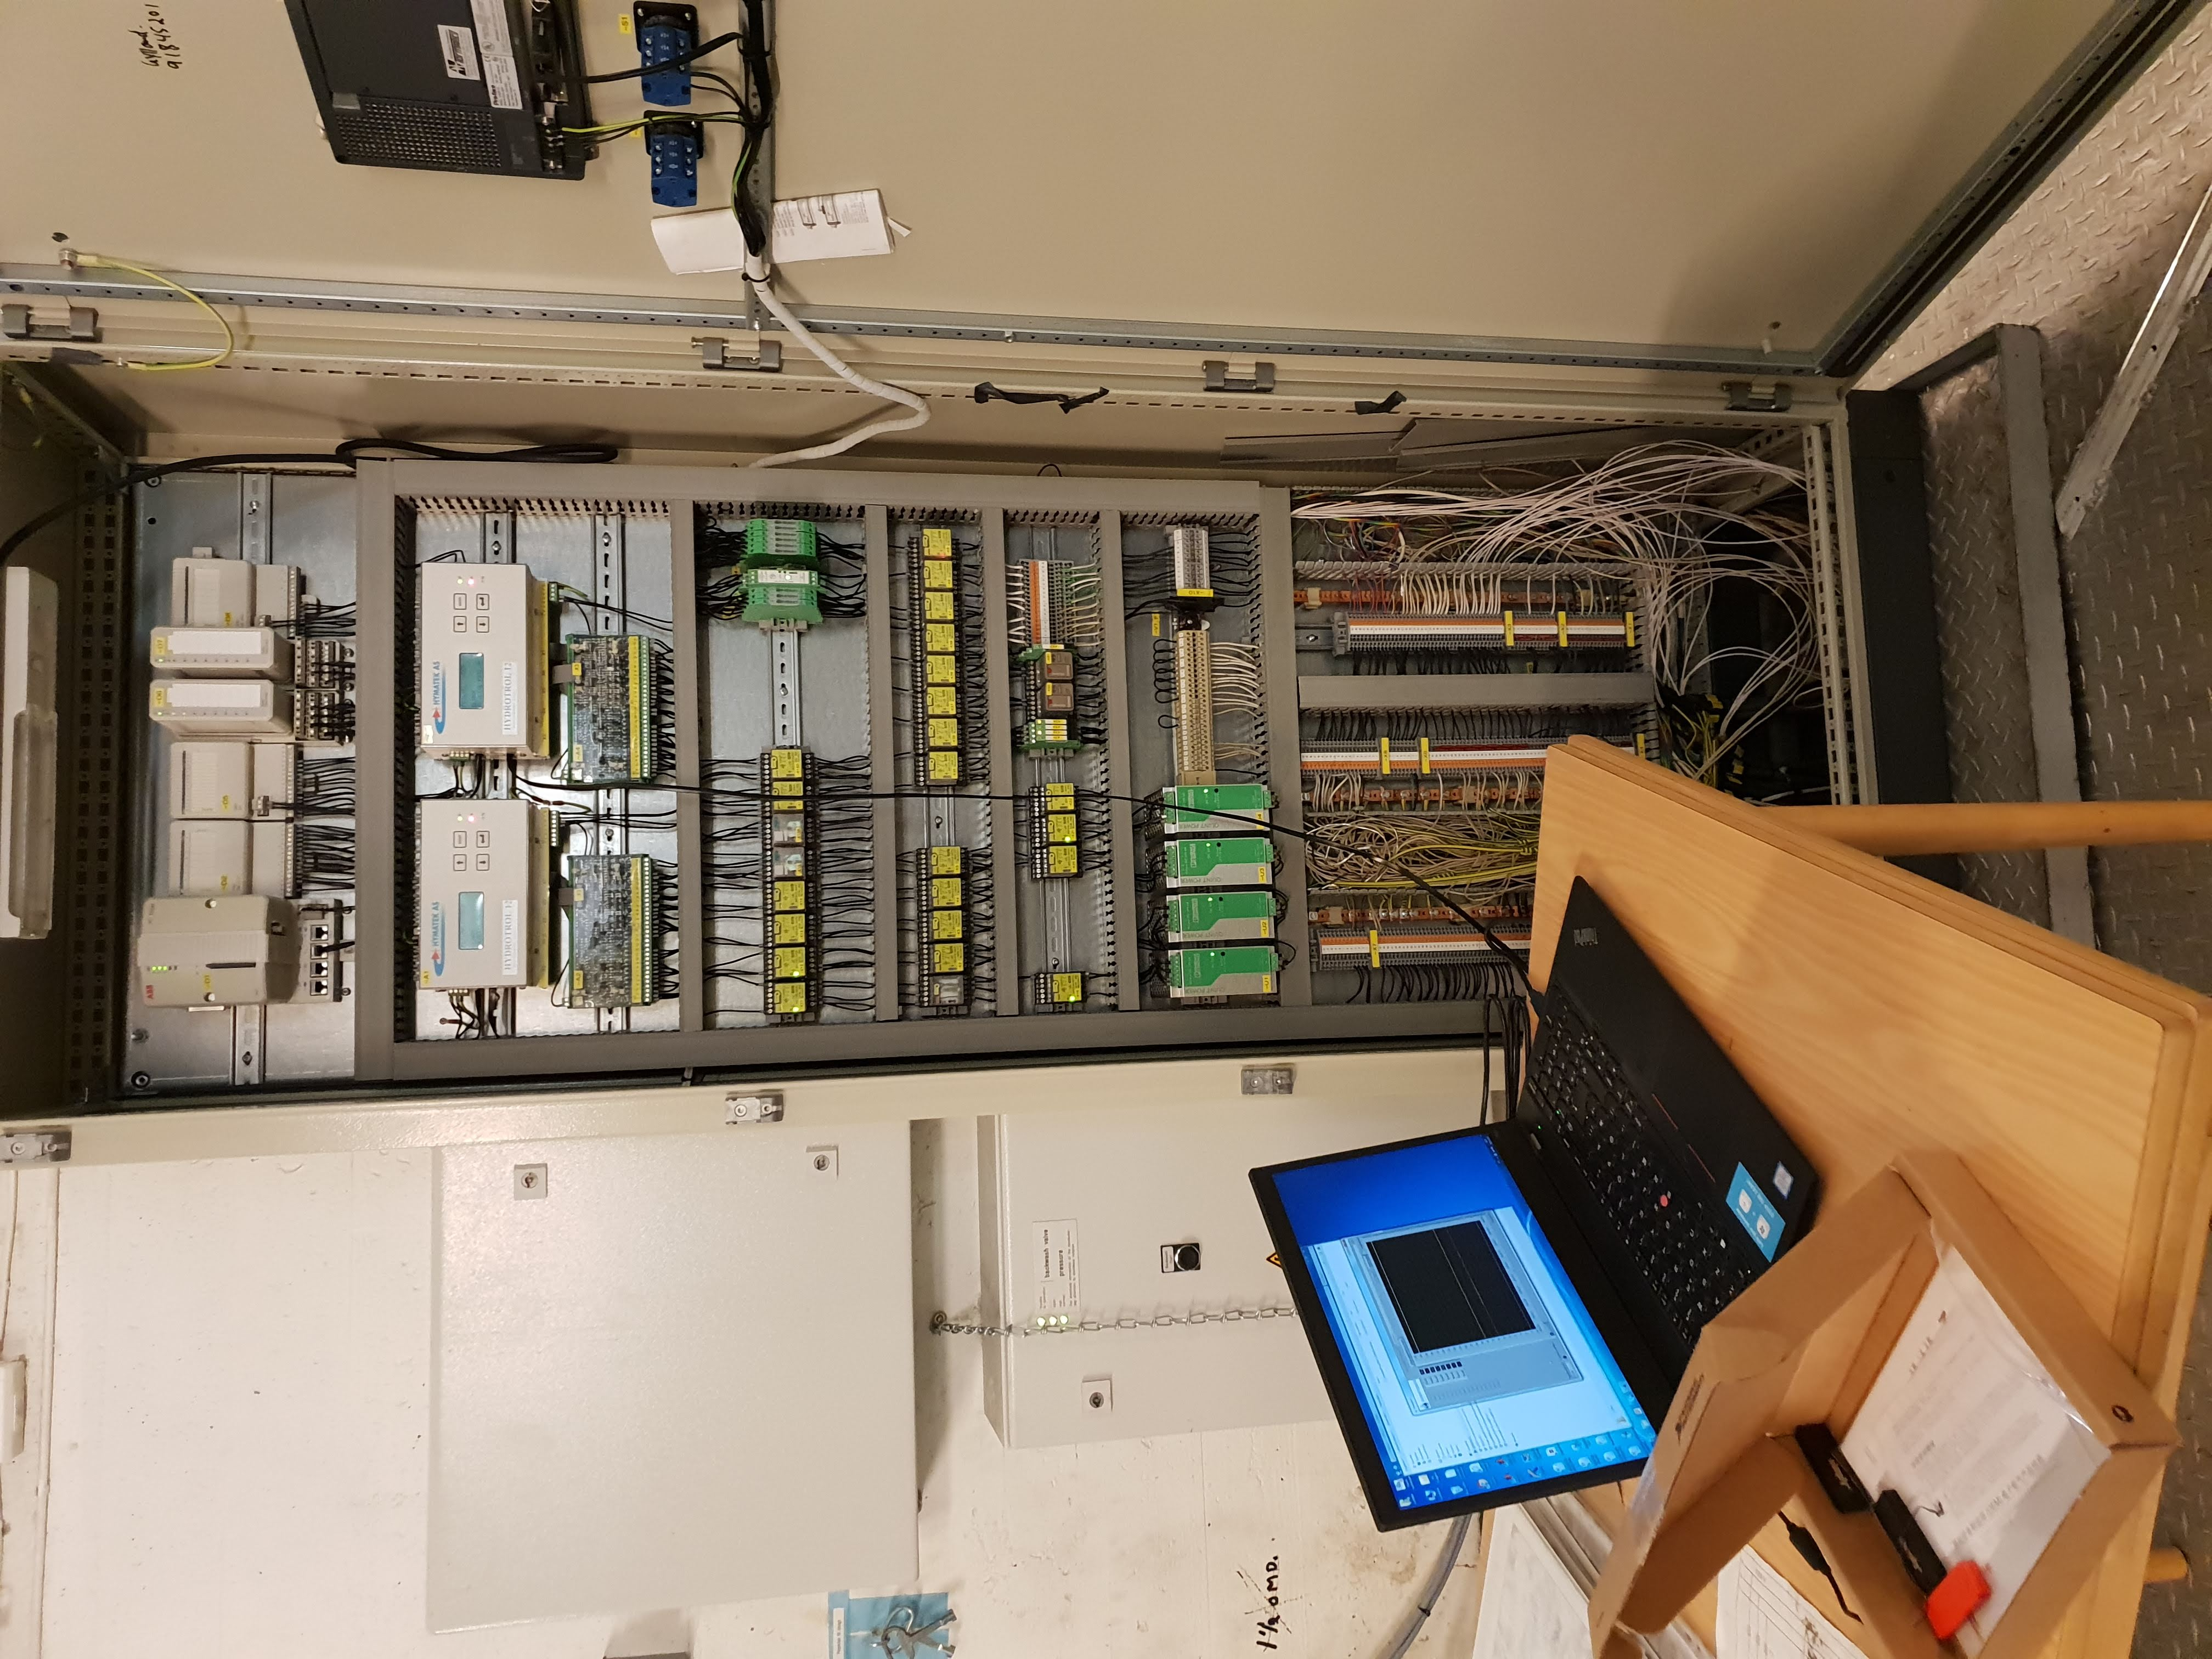
\includegraphics[angle=-90, origin= c, height=\textheight]{./pictures/hymatek.jpg}
		\end{column}
	\end{columns}
\end{frame}
\begin{frame}
	\frametitle{Measurement transformer}
	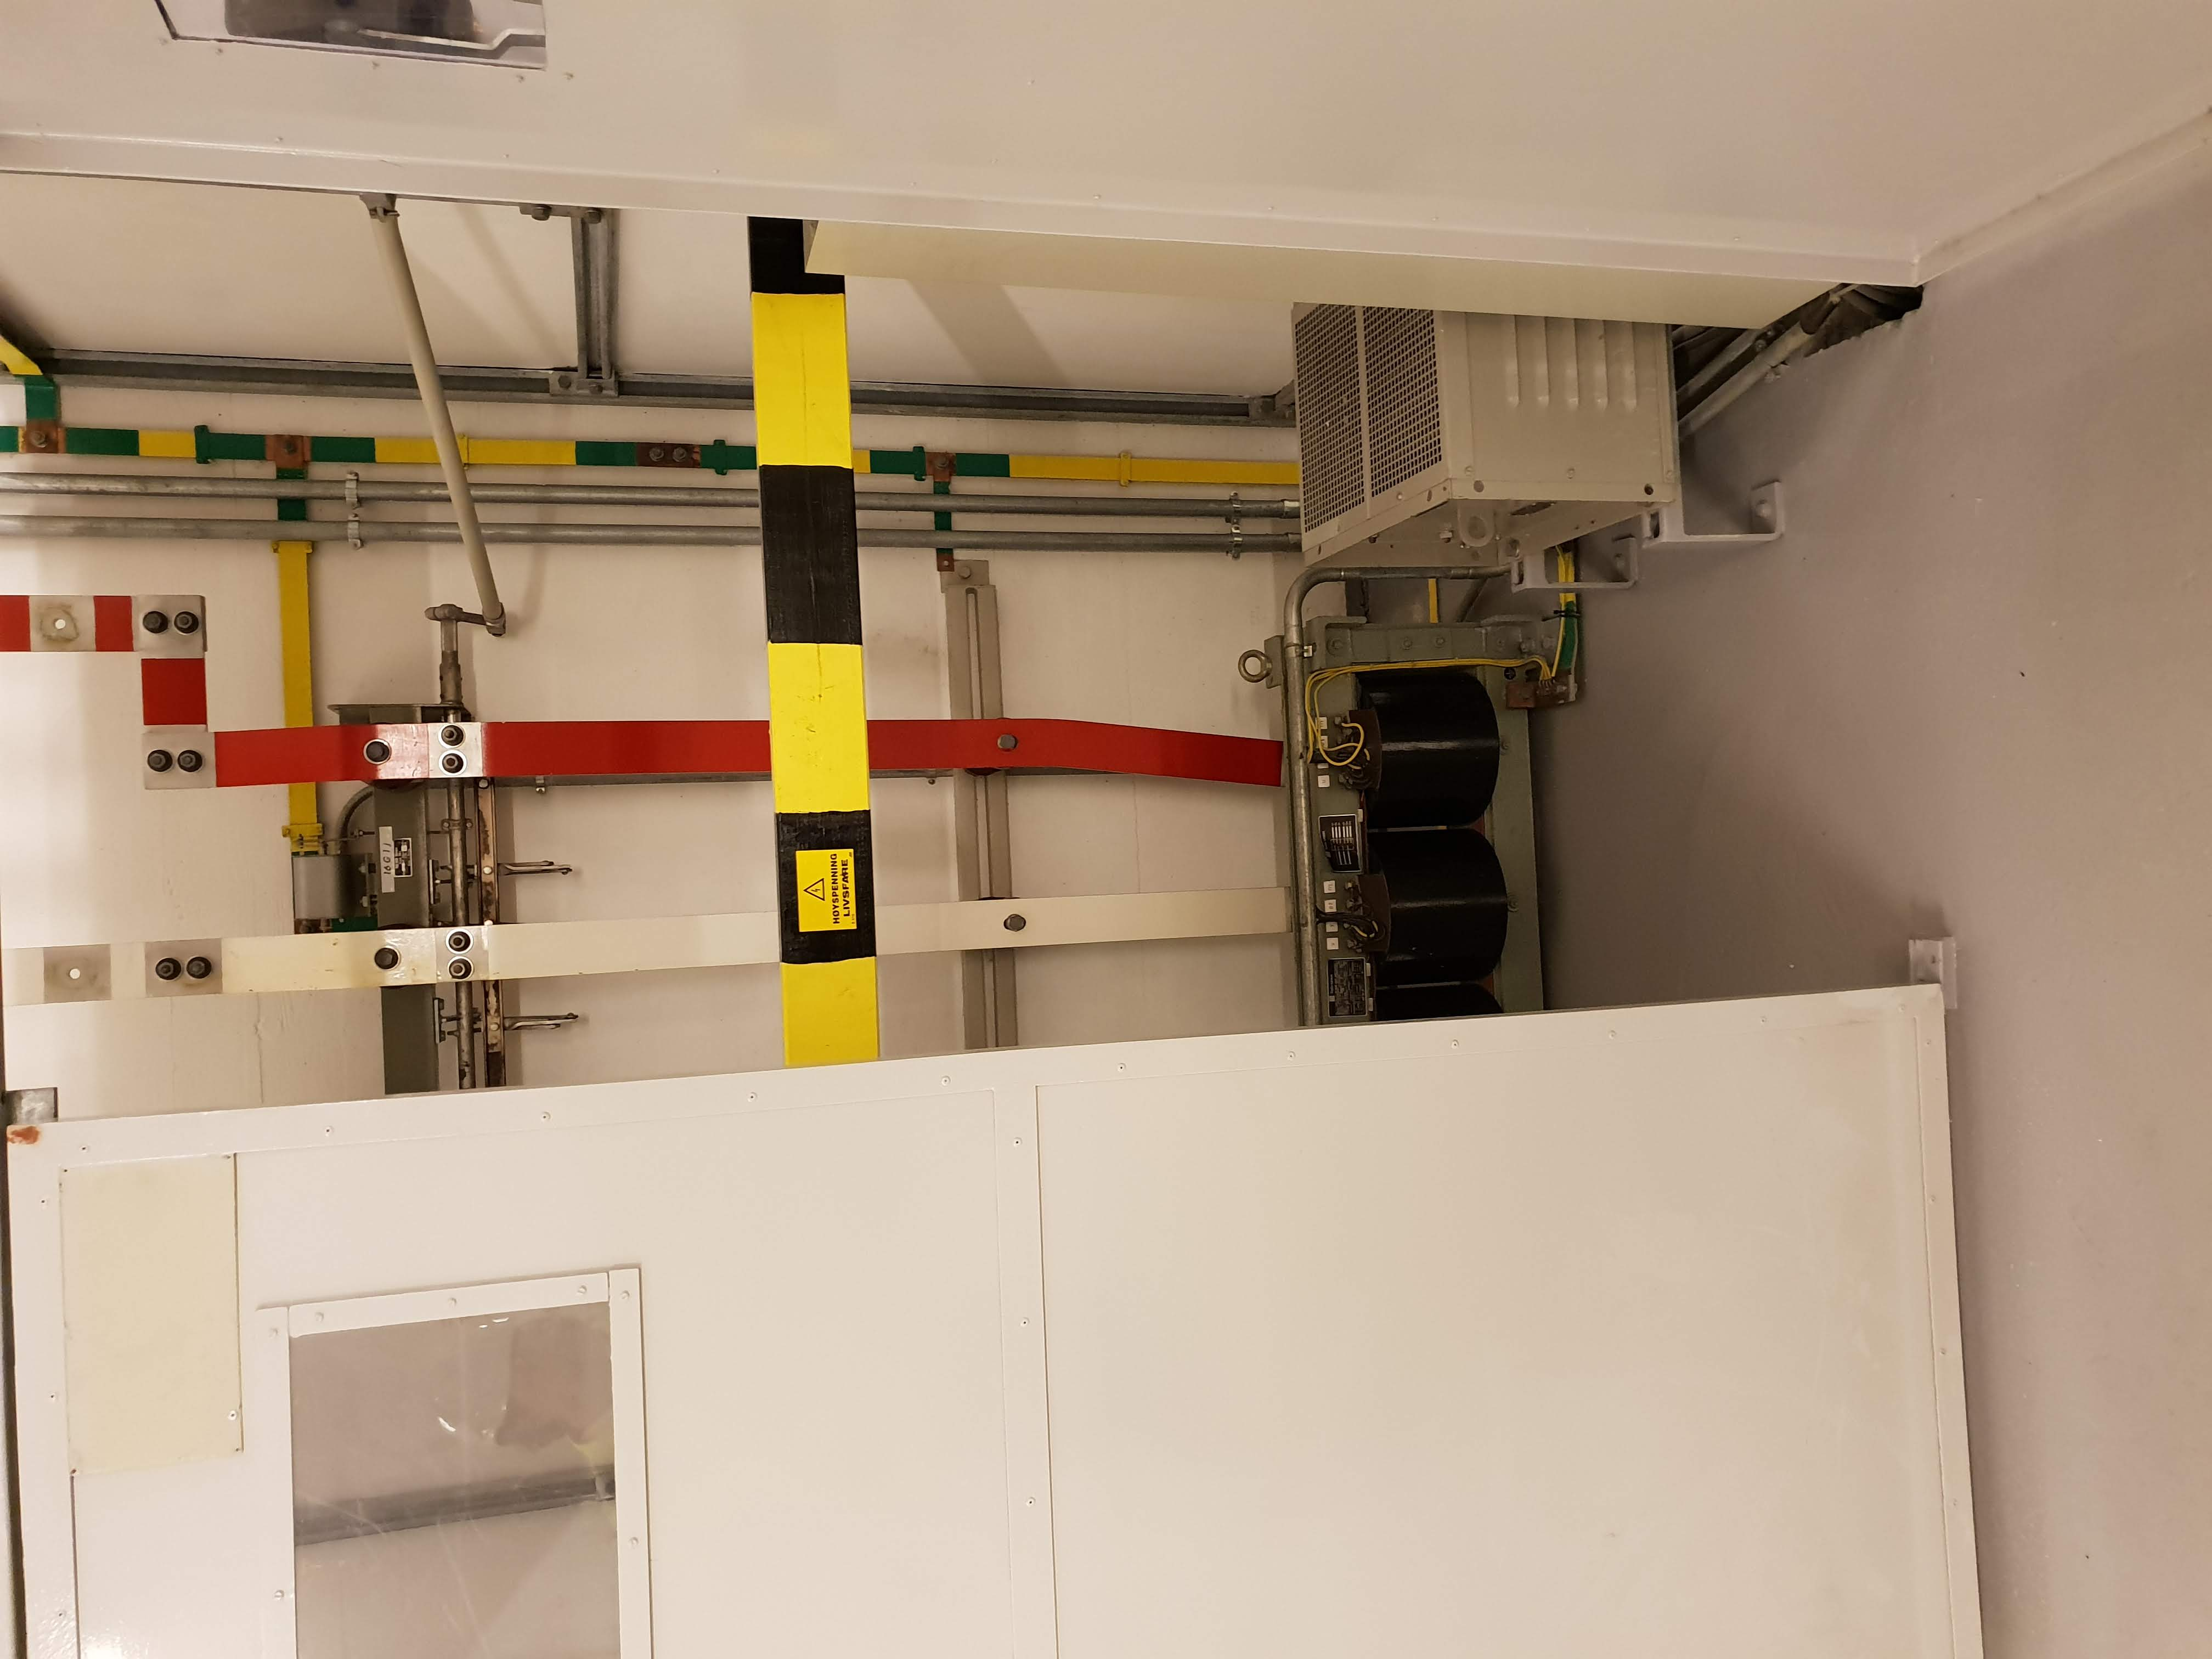
\includegraphics[angle=-90, origin=c, height=\textheight]{./pictures/trafo.jpg}
\end{frame}
\begin{frame}
	\frametitle{Example of dataset}
	\includegraphics[width=\textwidth]{./pictures/Grytten_signals.tikz}
\end{frame}
\begin{frame}
	\frametitle{Detecting a new tuning}
	\begin{columns}
		\begin{column}{0.65\textwidth}
			\includegraphics[width=\textwidth]{./pictures/Grytten_R_5.tikz}
		\end{column}
		\begin{column}{0.35\textwidth}
			\begin{equation*}
				G_1(s) = \frac{G_{J}}{1+G_p(s)G_J(s)}
			\end{equation*}
		\end{column}
	\end{columns}
	\includegraphics{./pictures/sys.tikz}
\end{frame}	
\begin{frame}
	\frametitle{Detecting droop changes}
	\begin{columns}
		\begin{column}{0.65\textwidth}
			\includegraphics[width=\textwidth]{./pictures/Grytten_new_PID.tikz}
		\end{column}
		\begin{column}{0.35\textwidth}
			\begin{equation*}
				G_1(s) = \frac{G_{J}}{1+G_p(s)G_J(s)}
			\end{equation*}
		\end{column}
	\end{columns}
	\includegraphics{./pictures/sys.tikz}
\end{frame}	
\begin{frame}
	\frametitle{Main Contributions}
	\begin{itemize}
		\item Proposal for alternative tests.
		\item Demonstrating that the proposed methods can detect parameter changes.
		\item Demonstrated that the industry proposed tests can be done easier.
	\end{itemize}
\end{frame}
